\part En la figura \ref{fig:triang_sem01}, el triángulo {\color{cielogris}XYZ} es semejante al triángulo {\color{strawberry}ABC}. ¿Cuál es el valor de $k$?

\begin{minipage}[t]{0.5\linewidth}
    \begin{figure}[H]
        \raggedright
        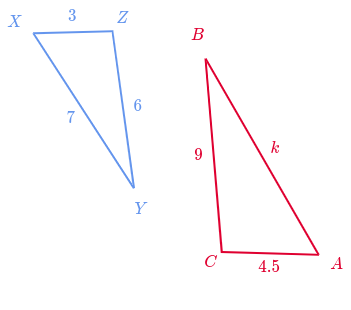
\includegraphics[width =0.8\linewidth ]{Images/triang_sem01}
        \caption{}
        \label{fig:triang_sem01}
    \end{figure}
\end{minipage}%
\begin{minipage}[t]{0.5\linewidth}
    \begin{solutionbox}{7cm}
        Los triángulos semejantes tienen lados proporcionales.

        $\Rightarrow$ podemos establecer proporciones equivalentes y resolver para $k$.

        $\therefore$
        \[
            \dfrac{k}{7} =\dfrac{9}{6} \]    y  \[k =10.5\]
    \end{solutionbox}
\end{minipage}
